\section{Моделирование предметной области и разработка функциональных
требований}

{
\renewcommand{\mathbf}[1]{#1}
\subsection{Сенсоры}

Для получения информации об окружающей среде используются различные сенсоры.

\subsubsection{Lidar}

\begin{figure}[h]
\centering
	\fbox{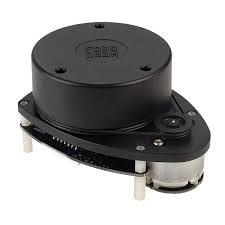
\includegraphics[width=9cm]{2d_lidar}}
\caption{2D Lidar}
\end{figure}

Сенсор Lidar выдаёт 2D снимок помещения -- облако точек в двумерной плоскости.
Используя облако точек, и зная позицию в которой снимок облака был совершён,
возможно реконструировать карту окружающего пространства на сетке. Если провести
отметить все клетки через которые прошёл луч за пустые, и отметить последнюю
клетку которую луч зацепил в качестве отмеченной, то получается 

\subsubsection{IMU}
Сенсор IMU (inertial measurement unit) даёт информацию об угловом и линейном
ускорении, что позволят определять текущее положение в пространстве.

\begin{figure}[h]
\centering
	\fbox{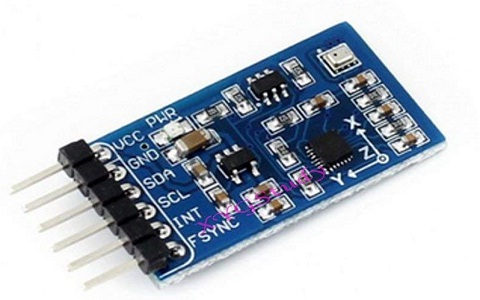
\includegraphics[width=9cm]{IMU}}
\caption{IMU}
\end{figure}

\subsubsection{GPS}
%\todo{По факту RTK может быть?}
Сенсор GPS выдаёт глобальную позицию в мировых координатах. Типичная точность
современных GPS-приёмников составляет 6-8 метров при хорошей видимости
спутников. 

\subsection{Алгоритмы фильтрации}
Используя сенсоры можно получать информацию о текущей позиции и скорости робота.
Сенсоры выдают значения с определённой погрешностью, из-за чего прямое
использование их значений приводит к неточной оценки позиции.

С помощью алгоритмов фильтрации несколько показаний с погрешностью сенсоров
можно комбинировать между собой и получать более точное приближение состояния.
Обычно в качестве состояния используется текущая позиция и ускорение.

Существует большое количество алгоритмов, позволяющие решать задачу оценки
состояния c учётом заданных ограничений (например, ограничений по доступным
вычислительным мощностям):

\begin{itemize}
	\item линейный фильтр Калмана (см. пункт $\ref{kf}$);
	\item расширенный фильтр Калмана (см. пункт $\ref{ekf}$);
	\item нелинейный фильтр Калмана (см. пункт $\ref{sec:ukf_info}$);
\end{itemize}

Каждый метод анализируется с точки зрения его математической основы и
применимости в задачах навигации.

\subsubsection{Фильтр Калмана}
\label{kf}
Фильтр Калмана -- рекурсивный алгоритм, обеспечивающий оптимальную оценку
состояния линейной динамической системы с нормально распределёнными шумами.
Предположение, что шум системы нормально распределён является ключевым. Динамику
системы в момент времени \( k \) можно описывается уравнением момент времени:
\begin{align}
    \mathbf{x}_k &= \mathbf{F}_k \mathbf{x}_{k-1} + \mathbf{B}_k \mathbf{u}_k + \mathbf{w}_k, \label{eq:kalman_state} \\
    \mathbf{z}_k &= \mathbf{H}_k \mathbf{x}_k + \mathbf{v}_k. \label{eq:kalman_meas}
\end{align}

\begin{explanationx}
	\item[где] \(\mathbf{x}_k\) -- вектор переменных состояния;
	\item \(\mathbf{z}_k\) -- вектор переменных измерений;
	\item \(\mathbf{u}_k\) -- управляющие переменные;
	\item \(\mathbf{w}_k\) шум процесса;
	\item \(\mathbf{v}_k \) -- шум измерений;
	\item \(\mathbf{F}_k\) -- матрица перехода состояния;
	\item \(\mathbf{B}_k\) -- матрица управления;
	\item \(\mathbf{H}_k\) -- матрица измерений.
\end{explanationx}

Переменные состояния (\(\mathbf{x}_k\)) описывают характеристики системы на временном шаге \( k \).
Переменные состояния полностью определяют её динамическое поведение.
Переменные измерения (\(\mathbf{z}_k\)) представляют наблюдаемые данные, получаемые от датчиков на шаге \( k \). 
Они описываются моделью измерений (см. уравнение \ref{eq:kalman_meas})
Управляющие переменные (\(\mathbf{u}_k\)) описывают внешние воздействия на систему, влияющие на её динамику.
Они входят в уравнение состояния и считаются известными, предоставляемыми системой управления.
Например, команды управления для перемещающегося средства.

Матрица перехода состояния \(\mathbf{F}_k\) описывает эволюцию состояния системы \(\mathbf{x}_k\) во времени без учёта управления и шума.
Матрица управления \(\mathbf{B}_k\) описывает влияние управляющего сигнала \(\mathbf{u}_k\) на состояние системы. Она также входит в уравнение состояния и имеет размер \(n \times m\), где \(m\) -- размерность \(\mathbf{u}_k\).

В идеальных условиях, шум процесса \(\mathbf{w}_k\) и шум измерений \(\mathbf{м}_k\)
полагаются равны 0. Шум процесса устанавливается в зависимости от степени
доверия системе и измерениям.

Все переменные, в зависимости от возможности произвести наблюдение за значением,
можно разделить на скрытые и явные зависимости.
К скрытым переменным относят:
\begin{itemize}
    \item переменные состояния $\mathbf{x}_k$; 
    \item шум процесса $\mathbf{w}_k$.
\end{itemize}

К явным переменным относят:
\begin{itemize}
    \item переменные измерений $\mathbf{z}_k$; 
    \item управляющие переменные $\mathbf{u}_k$; 
    \item шум измерений $\mathbf{v}_k$.
\end{itemize}

Работа фильтра Калмана основана на последовательном выполнении этапов предсказания (predict) и 
коррекции (update).

На этапе предсказания выполняется расчёт 
априорной оценки переменных состояния (см. уравнение \ref{x_predict})
и априорной оценки ковариация ошибка системы (см. уравнение \ref{p_predict}).
\begin{align}
\hat{\mathbf{x}}_{k|k-1} &= \mathbf{F}_k \hat{\mathbf{x}}_{k-1|k-1} + \mathbf{B}_k \mathbf{u}_k, \label{x_predict}\\
\mathbf{P}_{k|k-1} &= \mathbf{F}_k \mathbf{P}_{k-1|k-1} \mathbf{F}_k^T + \mathbf{Q}_k. \label{p_predict}.
\end{align}

Этап коррекции обновляет априорную оценку с учётом измерений, полученных с использованием датчиков.
Для этого вычисляются коэффициент усиления Калмана \(\mathbf(K)_k\) (см. уравнение \ref{kf_gain}),
апостериорная оценка состояния \(\mathbf{x}_{k|k}\) (см. уравнение \ref{x_update}),
и апостериорная ковариация ошибки \(\mathbf{P}_{k|k}\) (см. уравнение \ref{p_update}).

\begin{equation}
\label{kf_gain}
\mathbf{K}_k = \mathbf{P}_{k|k-1} \mathbf{H}_k^T (\mathbf{H}_k \mathbf{P}_{k|k-1} \mathbf{H}_k^T + \mathbf{R}_k)^{-1},
\end{equation}

\begin{equation}
\label{x_update}
\hat{\mathbf{x}}_{k|k} = \hat{\mathbf{x}}_{k|k-1} + \mathbf{K}_k (\mathbf{z}_k - \mathbf{H}_k \hat{\mathbf{x}}_{k|k-1}),
\end{equation}

\begin{equation}
\label{p_update}
\mathbf{P}_{k|k} = (\mathbf{E} - \mathbf{K}_k \mathbf{H}_k) \mathbf{P}_{k|k-1}.
\end{equation}
\\

Коэффициент \(\mathbf{K}_k\) балансирует доверие к модели и измерениям, снижая неопределённость.

\subsubsection{Расширенный фильтр Калмана (Extended Kalman Filter)}
\label{ekf}


Расширенный фильтр Калмана (EKF) адаптирует фильтр Калмана (KF) для нелинейных систем:

\begin{align}
    \mathbf{x}_k &= \mathbf{f}(\mathbf{x}_{k-1}, \mathbf{u}_k) + \mathbf{w}_k, \\
    \mathbf{z}_k &= \mathbf{h}(\mathbf{x}_k) + \mathbf{v}_k.
\end{align}

Линеаризация выполняется с помощью матриц Якоби \(\mathbf{F}_k = \frac{\partial \mathbf{f}}{\partial \mathbf{x}}\big|_{\hat{\mathbf{x}}_{k-1|k-1}}\) и \(\mathbf{H}_k = \frac{\partial \mathbf{h}}{\partial \mathbf{x}}\big|_{\hat{\mathbf{x}}_{k|k-1}}\). Этапы предсказания и коррекции аналогичны фильтру Калмана, но ошибки линеаризации снижают точность при сильной нелинейности.

\subsubsection{Нелинейный фильтр Калмана (Unscented Kalman Filter)}
\label{sec:ukf_info}

UKF использует сигма-точки для обработки нелинейностей без линеаризации. Сигма-точки генерируются на основе \(\hat{\mathbf{x}}_{k-1|k-1}\) и \(\mathbf{P}_{k-1|k-1}\), затем распространяются через \(\mathbf{f}\) и \(\mathbf{h}\):
\begin{align}
    \hat{\mathbf{x}}_{k|k-1} &= \sum w_i \mathbf{f}(\mathbf{x}_i), \\
    \mathbf{P}_{k|k-1} &= \sum w_i (\mathbf{f}(\mathbf{x}_i) - \hat{\mathbf{x}}_{k|k-1})(\mathbf{f}(\mathbf{x}_i) - \hat{\mathbf{x}}_{k|k-1})^T + \mathbf{Q}_k.
\end{align}
Для состояния \(\mathbf{x}_{k-1|k-1}\) с оценкой 
\(\hat{\mathbf{x}}_{k-1|k-1}\) и ковариацией \(\mathbf{P}_{k-1|k-1}\) 
генерируется \(2n + 1\) сигма-точек, где \(n\)  -- это размерность вектора состояний \(\mathbf{x}_k\).
Для генерации точек используется следующий алгоритм:

\begin{itemize}
    \item вычисление масштабирующего параметра:
    \[
    \lambda = \alpha^2 (n + \kappa) - n,
    \]
    где \(\alpha\) (\(10^{-3} \leq \alpha \leq 1\)) контролирует разброс, \(\kappa\) (обычно \(3 - n\)) -- параметр настройки.
    \item генерация сигма-точек:
    \[
    \mathbf{x}_{k-1}^{(0)} = \hat{\mathbf{x}}_{k-1|k-1},
    \]
    \[
    \mathbf{x}_{k-1}^{(i)} = \hat{\mathbf{x}}_{k-1|k-1} + (\sqrt{(n + \lambda) \mathbf{P}_{k-1|k-1}})_i, \quad i = 1, \dots, n,
    \]
    \[
    \mathbf{x}_{k-1}^{(i)} = \hat{\mathbf{x}}_{k-1|k-1} - (\sqrt{(n + \lambda) \mathbf{P}_{k-1|k-1}})_{i-n}, \quad i = n+1, \dots, 2n,
    \]
    где \((\sqrt{(n + \lambda) \mathbf{P}_{k-1|k-1}})_i\) -- \(i\)-й столбец разложения Холецкого.
    \item назначение весов:
    \[
    w_m^{(0)} = \frac{\lambda}{n + \lambda}, \quad w_m^{(i)} = \frac{1}{2(n + \lambda)}, \quad i = 1, \dots, 2n,
    \]
    \[
    w_c^{(0)} = \frac{\lambda}{n + \lambda} + (1 - \alpha^2 + \beta), \quad w_c^{(i)} = \frac{1}{2(n + \lambda)}, \quad i = 1, \dots, 2n,
    \]
    где \(\beta \approx 2\) для нормального распределения.
\end{itemize}

В общем случае, UKF работает более точно, чем EKF:
\begin{itemize}
    \item высокая точность при сильной нелинейности, так как сигма-точки лучше аппроксимируют распределение;
    \item отсутствие необходимости вычислять производные, что упрощает реализацию для сложных функций.
\end{itemize}

\subsection{AHRS}
\label{subsec:ahrs}

Система ориентации и курса (Attitude and Heading Reference System или AHRS) предназначена для оценки
ориентации объекта: углов крена (roll), тангажа (pitch) и рысканья (yaw).
В задачах навигации, подобных тем, где применяются фильтр частиц (PF) или фильтры Калмана,
AHRS играет ключевую роль в определении ориентации.
Основные источники данных, для которых используется AHRS: 
\begin{itemize}
    \item гироскопы (\(\boldsymbol{\omega} = [\omega_x, \omega_y, \omega_z]^T\)) для измерения угловой скорости;
    \item акселерометры (\(\mathbf{a} = [a_x, a_y, a_z]^T\)) для оценки крена и тангажа через вектор силы тяжести;
    \item магнитометры (\(\mathbf{m} = [m_x, m_y, m_z]^T\)) для определения рысканья относительно магнитного севера.
\end{itemize}

Ориентация представляется в системе кватернионом \(\mathbf{q} = [q_0, q_1, q_2, q_3]^T\), что позволяет
избежать блокировки кардана (gimbal lock).

Применение AHRS ограничивается рядом внешних условий:

\begin{enumerate}[label=\arabic*]
    \item Наличие магнитных помех искажают показания магнитометров.
    \item Дрейф гироскопов требует внешней коррекции. Использование алгоритмов фильтрации
	    с AHRS позволяет произвести корректировку дрейфа гироскопов.
    \item AHRS не моделирует положение и линейную скорость.
\end{enumerate}

\subsection{Оценка измерений в AHRS}

Для оценки ориентации в AHRS принято использовать один из двух алгоритмов: фильтр Маджвика или фильтр Махони.

\subsubsection{Фильтр Маджвика}

Фильтр Маджвика использует градиентный спуск для минимизации ошибки гироскопа 
с коррекцией от акселерометра и магнитометра. Он оценивает кватернион ориентации
\(\mathbf{q}_t\) путём численного интегрирования:

\begin{equation}
    \dot{\mathbf{q}}_t = \dot{\mathbf{q}}_{\omega, t} - \beta \dot{\mathbf{q}}_{\epsilon, t},
\end{equation}
где
    \(\dot{\mathbf{q}}_{\omega, t} = \frac{1}{2} \mathbf{q}_{t-1} \otimes \begin{bmatrix} 0 \\ 
    \boldsymbol{\omega}_t \end{bmatrix}\) -- изменения ориентации от гироскопа \(\boldsymbol{\omega}_t\);
    \(\dot{\mathbf{q}}_{\epsilon, t}\) -- 
    численное значение ошибки, вычисленное градиентным спуском из данных акселерометра 
    (\(\mathbf{a}_t\)) и магнитометра (\(\mathbf{m}_t\));
    \(\beta\) -- коэффициент доверия к фильтру ($\beta \in [0.1, 1]$).

Основными преимуществами фильтра Маджвика являются:
\begin{itemize}
	\item высокая точность вычисления ориентации;
	\item эффективная компенсация дрейфа гироскопа.
\end{itemize}

\subsubsection{Фильтр Махони}

Фильтр Махони основан на нелинейном комплементарном фильтре на группе \(SO(3)\).
Он минимизирует ошибку между измеренными и эталонными векторами с помощью пропорционально-интегрального (PI)
компенсатора. Ориентация обновляется как:

\begin{equation}
    \dot{\mathbf{q}}_t = \frac{1}{2} \mathbf{q}_t \otimes \begin{bmatrix} 0 \\ \boldsymbol{\omega}_t + \mathbf{e}_t \end{bmatrix},
\end{equation}
где
    \(\mathbf{e}_t = k_P \boldsymbol{\omega}_{\text{err}} + k_I \int \boldsymbol{\omega}_{\text{err}} \, dt\) --
    коррекция, основанная на ошибке \(\boldsymbol{\omega}_{\text{err}}\), 
    вычисленной как векторное произведение измеренных и предсказанных векторов.
    \(k_P \approx 1\), \(k_I \approx 0.3\) -- PI-компенсатора.

К основным преимуществам фильтра Махони относят:
\begin{itemize}
	\item быстрая сходимость;
	\item низкая вычислительная сложность.
\end{itemize}

Фильтр требует тщательного выбора параметров \(k_P\), \(k_I\). По сравнению с фильтром Маджвика, 
фильтр Махони хуже оценивает ориентацию в пространстве.


Таким образом, оба фильтра имеют место быть для различных условий применения.
Фильтр Маджвика предоставляет большую точность на низкой частоте отправке данных.
Фильтр Махони используются на системах с ограниченной вычислительной мощностью.

% \subsection{Алгоритмы SLAM}
% В подразделе \ref{sec:ros_analysys} шла речь о двух основных типов алгоритмов.
% Более ранние алгоритмы, основанные на фильтрах Байеса, и более новые методы,
% основанные на графах.
% Рассмотрим сначала подходы основанные на фильтрах Байеса.
%
% \subsubsection{Фильтры байеса}
% % NN generated
%
% \subsubsection{SLAM основанный на графах}

\subsection{Сетка занятости (Occupancy grid)}

Карта занятости (Occupancy Grid) в двумерном представлении является сеткой,
разделяющей пространство на регулярные ячейки, каждая из которых отражает
состояние окружающей среды. Каждая ячейка хранит информацию о вероятности
наличия препятствия, принимая значения, соответствующие состояниям: занята
(препятствие присутствует), свободна (доступно для движения) или неизвестна
(данные отсутствуют). Карты формируются на основе данных сенсоров, и обновляются
в реальном времени, позволяя роботу адаптироваться к динамическим изменениям в
среде.

Двумерные карты занятости широко применяются в мобильной робототехнике для задач
навигации и планирования маршрутов. Они обеспечивают простое и эффективное
представление окружающей среды, позволяя роботу определять свободные пути,
избегать препятствий и строить оптимальные траектории движения. Благодаря своей
структуре, такие карты легко интегрируются в алгоритмы локализации и
картирования (SLAM), что делает их ключевым инструментом для автономного
передвижения мобильных роботов в сложных условиях.

\subsection{Построение карты}

\subsubsection{ICP}
Iterative Closest Point (ICP) -- классический алгоритм регистрации облаков
точек, широко используемый в компьютерном зрении и робототехнике для точного
выравнивания двух наборов данных, полученных с помощью лидаров или других
3D-сканеров.

Основная цель ICP -- расстояние между двумя облаками точек:
фиксированным эталонным (reference) и подвижным (source), который необходимо
трансформировать (сдвинуть и повернуть) так, чтобы максимально приблизить к
эталону. Алгоритм работает итеративно, последовательно уточняя параметры
преобразования.

1 Алгоритм начинается с предварительной оценки преобразования, которое
приблизительно совмещает исходное облако с эталонным. Качество начального
приближения существенно влияет на результат, поскольку ICP может сойтись к
локальному минимуму.
    
2 Для каждой точки подвижного облака находится ближайшая точка в эталонном
облаке по евклидову расстоянию. Для ускорения поиска обычно используется
структура данных k-d дерево.
    
3 На основе найденных пар точек вычисляется оптимальное преобразование (смещение
и поворот), минимизирующее среднеквадратичное расстояние между соответствующими
точками. Часто применяется метод наименьших квадратов.
    
4 Подвижное облако точек трансформируется с использованием найденного
преобразования.
    
5 Шаги поиска соответствий и оценки преобразования повторяются до тех пор, пока
изменение ошибки не станет меньше заданного порога или не будет достигнуто
максимальное число итераций.

\subsubsection{Особенности и ограничения ICP}
\begin{itemize}
	\item ICP чувствителен к качеству начального приближения и может застревать
		в локальных оптимумах;
	\item алгоритм хорошо работает при небольших смещениях и поворотах между
		сканами;
	\item существует множество вариантов ICP, включая point-to-point (точка к
		точке) и point-to-plane (точка к плоскости), последний из которых лучше
		подходит для структурированных поверхностей;
\end{itemize}

ICP является базовым инструментом для регистрации 2D и 3D данных в задачах SLAM,
реконструкции объектов и навигации мобильных платформ, особенно когда требуется
точное совмещение облаков точек, полученных с разных позиций или в разное время.

Таким образом, ICP -- эффективный и относительно простой алгоритм,
обеспечивающий точное выравнивание облаков точек за счёт итеративного уточнения
преобразования между ними.

В алгоритме Iterative Closest Point (ICP) задача сводится к поиску оптимального
жёсткого преобразования (поворота и сдвига), которое минимизирует сумму
квадратов расстояний между соответствующими точками двух облаков. Для решения
этой задачи на каждом шаге, когда соответствия между точками уже известны,
широко применяется метод сингулярного разложения матриц (SVD, Singular Value
Decomposition).

\subsubsection{CSM}
Correlative scan matching (CSM) -- метод регистрации сканов лидара, используемый
в робототехнике для определения относительного положения робота на карте. Его
ключевое преимущество -- устойчивость к локальным минимумам и высокая точность, что делает его критически важным для задач одновременной локализации и построения карт (SLAM).

Принцип работы CSM заключается в поиске оптимального преобразования (сдвига и поворота) между двумя наборами точек (сканами), при котором достигается максимальное совпадение между ними. В отличие от итеративных методов, таких как ICP (Iterative Closest Point), которые зависят от начального приближения и могут застревать в локальных оптимумах, CSM осуществляет дискретный перебор возможных трансформаций в заданном диапазоне. Для каждой трансформации вычисляется функция качества совпадения, основанная на вероятностной модели окружающей среды или на карте стоимости.

Алгоритм строит карту стоимости, где каждой точке пространства соответствует значение, отражающее вероятность её принадлежности к объекту или свободному пространству. Затем, перебирая множество вариантов сдвигов и поворотов, CSM вычисляет суммарную оценку совпадения между текущим сканом и картой. Оптимальное преобразование выбирается как то, при котором эта оценка максимальна.

Преимущества CSM включают:
\begin{itemize}
	\item глобальный поиск решения, минимизирующий риск сходимости к локальным минимумам;
	\item высокую устойчивость к шуму и ошибкам сенсорных данных;
	\item возможность работы при значительной начальной неопределённости положения.
\end{itemize}

CSM широко применяется в задачах одновременной локализации и построения карт (SLAM), особенно для коррекции ошибок одометрии и закрытия петель, что позволяет значительно повысить точность и надёжность навигационных систем мобильных роботов.


\subsection{Построение маршрута}
Глобальные планировщики предназначены для построения маршрута от начальной точки
до цели в известной или частично известной среде, обычно представленной в виде
графа или сетки. В качестве глобальных планировщиков используют:
\begin{itemize}
	\item алгоритм Дейкстры;
	\item алгоритм A*;
	\item алгоритм RRT.
\end{itemize}

\subsubsection{Алгоритм Дейкстры}

Алгоритм Дейкстры служит для поиска кратчайшего пути в графе с неотрицательными
весами рёбер. Начиная с начальной вершины, алгоритм последовательно обновляет
расстояния до всех остальных вершин, выбирая на каждом шаге вершину с
минимальным текущим расстоянием. Для выбранной вершины проверяются её соседи, и
расстояния до них обновляются, если найден более короткий путь. Процесс
продолжается до обработки всех вершин или достижения цели.

Математически алгоритм минимизирует расстояние до вершины $v$ по формуле:
\begin{equation}
d[v] = \min_{u \in V} \{ d[u] + w(u, v) \},
\end{equation}

\begin{explanationx}
\item[где] $d[v]$ -- кратчайшее расстояние от начальной вершины до $v$;
\item $w(u, v)$ -- вес ребра между вершинами $u$ и $v$.
\end{explanationx}

Алгоритм гарантирует оптимальность пути,
но для больших графов требует значительных вычислений,
с временной сложностью $O((V + E) \log V)$ при использовании кучи.

\subsubsection{Алгоритм A*}
Алгоритм A* улучшает подход Дейкстры,
добавляя эвристическую функцию для ускорения поиска.
Каждая вершина оценивается по сумме стоимости пути от начальной точки ($g(v)$)
и эвристической оценки расстояния до цели ($h(v)$).
Выбирается вершина с минимальной суммой $f(v) = g(v) + h(v)$.
Эвристика должна быть допустимой, то есть не переоценивать истинное расстояние: $h(v) \leq h^*(v)$,
где $h^*(v)$ -- реальное расстояние до цели.

Логику алгоритма можно описать формулой:
\begin{equation}
f(v) = g(v) + h(v).
\end{equation}

A* эффективен для планирования в сетках или графах,
особенно при использовании точной эвристики для сокращения количество проверяемых вершин.

\subsubsection{RRT (Rapidly-exploring Random Tree)}
RRT -- алгоритм для планирования маршрутов в непрерывных высокомерных
пространствах. Алгоритм строит дерево, начиная с начальной конфигурации, путём
случайной выборки точек в конфигурационном пространстве. Для каждой случайной
точки находится ближайший узел дерева, и к нему добавляется новая конфигурация
на расстоянии $\delta$ в направлении случайной точки, если она свободна от
препятствий. Процесс повторяется до достижения цели или превышения лимита
итераций.

Упрощённо работу алгоритма можно описать формулой:
\begin{equation}
q_{\text{new}} = q_{\text{near}} + \delta \cdot \frac{q_{\text{rand}} - q_{\text{near}}}{\| q_{\text{rand}} - q_{\text{near}} \|}.
\end{equation}

RRT вероятностно полный, но не обеспечивает оптимальность пути.

\subsection{Исполнение маршрута}
Алгоритмы производящие исполнение маршрута называются локальные планировщики.
Они планируют следующий шаг в изменении скорости, который потом конвертируется в
команды управления отправляемые на шасси.
Локальные планировщики корректируют движение робота в реальном времени, учитывая
динамику и локальные препятствия.

\subsubsection{DWA (Dynamic Window Approach)}
DWA предназначен для выбора оптимальной пары скоростей (линейной и угловой) с
учётом кинематических ограничений движущегося объекта. Алгоритм формирует
множество допустимых скоростей (динамическое окно), ограниченных текущим
состоянием и ускорениями:

\begin{equation}
W_d = \{ (v, \omega) \mid v \in [v_{\min}, v_{\max}],	\omega \in [\omega_{\min}, \omega_{\max}] \}.
\end{equation}

Для каждой пары скоростей моделируется траектория,
оцениваемая по ориентации к цели, расстоянию до препятствий и величине скорости.
Выбирается пара скоростей, минимизирующая целевую функцию $G(v, \omega)$:

\begin{equation}
(v^*, \omega^*) = \min_{(v, \omega) \in W_d} G(v, \omega),
\end{equation}

DWA активно используются для дифференциальных роботов. Но основным недостатком алгоритма
является проблема застревания в локальных минимумах целевой функции.

\subsubsection{TEB (Timed Elastic Band)}

TEB оптимизирует траекторию, представляя её как эластичную ленту,
которая деформируется для минимизации энергетический потерь на перемещение.
Траектория состоит из набора конфигураций (состояний) $\{q_1, q_2, \dots, q_n\}$, 
соединённых временными интервалами $\Delta T_i$. 

Алгоритм TEB оптимизирует эти конфигурации и интервалы, минимизируя целевую функцию:
\begin{equation}
	J(B) = \sum_{i=1}^{n-1} \left( w_1 \| q_{i+1} - q_i \|^2 + w_2 \Delta T_i^2 + w_3 \sum_{\text{obj}} \text{obj}(q_i, \text{p})^{-2} \right),
\end{equation}
где первый член обеспечивает компактность траектории, 
второй -- минимизацию времени, 
а третий -- избегание препятствий.

Конфигурации учитывают кинематические ограничения, такие как максимальная скорость:

\begin{equation}
v_i = \frac{q_{i+1} - q_i}{\Delta T_i}, \quad \| v_i \| \leq v_{\max}.
\end{equation}

По сравнению с DWA, TEB требует большей вычислительной сложностью,
но позволяет описать модель перемещения более точно. 

\subsection{Общие сведения и требования к работе программного средства}

% \subsection{Описание функциональности программного средства}
%
% \todo{USECASE диаграмма}
% \subsection{Спецификация функциональных требований}

- Моделируем навигацию
- Occupancy grid
- Надо переместится в указанную точку на карте
- Способ указывания точки на карте

% \todo{ Если цель переместится в указанную точку, для этого надо построить
% маршрут, чтобы построить маршрут нужна карта, чтобы построить карту используем
% позицию и показания с сенсоров и метод SLAM }

\subsection{Разработка функциональных требований к проектируемому программному
средству}
% WATER
	Для успешной реализации системы мобильной навигации необходимо четко
	определить и описать функциональные требования, которые будут обеспечивать
	эффективность и точность работы системы. Эти требования являются основой для
	проектирования и разработки как аппаратной, так и программной части системы.
	В данном разделе мы рассмотрим ключевые аспекты, которые должны быть учтены
	при разработке функциональных требований для мобильной навигации, включая
	работу с картами, выполнение маршрутов и интеграцию различных сенсоров.

Система должна:
\begin{itemize}
	\item получать данные с сенсоров IMU, GPS, Lidar;
	\item обрабатывать полученные данные и определять текущую позицию;
	\item строить карту окружающей среды;
	\item строить и выполнять маршут перемещаясь в указанную позицию;
	\item сохранять и загружать построенную карту между запусками;
\end{itemize}

\subsection{Разработка технических требований к программному средству}

Разрабатываемое программное решение должно обеспечивать корректное
функционирование при развёртывании на компьютерном модуле BananaPi CM4, или
на модуле со следующими техническими характеристиками:

\begin{itemize}
	\item оперативная память 4 Гбайт или более;
	\item amlogic A311D шести ядерный процессов с четырьмя Arm Cortex-A73
		ядрами, двумя Arm Cortex-A53 ядрами, или более быстродействующий
		процессор;
	\item доступный объём дискового пространства 5 Гбайт. %20mb на самом деле
\end{itemize}
